\documentclass{article}
\usepackage[utf8]{inputenc}
\usepackage[margin=1in]{geometry}

\title{518 - Assignment 2}
\author{Victor Zhang, Bharti Mehta}
\date{May 3rd, 2021}

\usepackage[utf8]{inputenc}
\usepackage{amsmath}
\usepackage{amsfonts}
\usepackage{natbib}
\usepackage{graphicx}
% \usepackage{changepage}
\usepackage{amssymb}
\usepackage{xfrac}
% \usepackage{bm}
% \usepackage{empheq}
\usepackage{dirtytalk}
\usepackage{tikz}
\usepackage{hyperref}

\newcommand{\contra}{\raisebox{\depth}{\#}}

\newenvironment{myindentpar}[1]
  {\begin{list}{}
          {\setlength{\leftmargin}{#1}}
          \item[]
  }
  {\end{list}}

\pagestyle{empty}

\tikzset{every picture/.style={line width=0.75pt}} %set default line width to 0.75pt

\hypersetup{
    colorlinks=true,
    linkcolor=blue,
    filecolor=magenta,      
    urlcolor=cyan,
}

\urlstyle{same}

\begin{document}

\maketitle
% \begin{center}
% {\huge Econ 482 \hspace{0.5cm} HW 3}\
% {\Large \textbf{Victor Zhang}}\
% {\Large February 18, 2020}
% \end{center}

\section{Introduction}
The purpose of this assignment is to augment our existing thread implementation with a memory management system. The design specifies a \say{main memory} size of 8MB and \say{disk} size of 16MB. Because of nice properties we can exploit with these sizes, we build our memory management system under the strict assumption of 8MB main memory and 16MB disk. That is, it is not easily scalable to any larger size of memory or disk. The drawback is obvious, but the advantage is this allows us to be extremely compact in our metadata. In addition, we work under the assumption of 4k pages. Since this is essentially the the standard everywhere (unless using hugepages), we feel this is a reasonable assumption to make.

\section{Phase 1}
For this phase, the main task is to efficiently allocate memory within a page.
We use a segmented paging strategy implemented using a linkedlist. We allocate
in blocks of size 64 bytes (a typical cache line), meaning there are
$4096/64 = 64$ blocks in each page. For each segment, we keep one byte of
metadata. Figure \ref{fig:segment_metadata} shows this. The top bit represents
the status of the segment, \verb|1| for occupied, \verb|0| for free. The second bit represents whether the segment is the last segment in the page, \verb|1| if it is, \verb|0| if it isn't/ The rest of
the bits represent the length of this segment. But a segment can have length 64,
which requires 7 bits to represent! We solve this problem by introducing
\textit{normalized lengths}. Since each segment will have length at least 1, it
makes no sense to start counting from 1. A normalized length of 0 will
correspond with an actual length of 1 block. In general, a normalized length of
$k$ corresponds with an actual length of $k+1$ blocks. This  allows us to
represent the length of a completely free page (64 blocks) in 6 bits instead of
8. So remarkably, we can fit all of our necessary metadata within one byte.

\begin{figure}
\centering
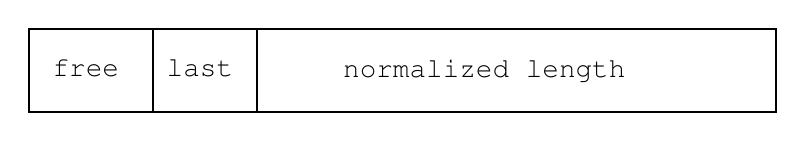
\begin{tikzpicture}[x=0.75pt,y=0.75pt,yscale=-1,xscale=1]
\draw   (190,50) -- (550,50) -- (550,90) -- (190,90) -- cycle ;
\draw    (250,50) -- (250,90) ;
\draw    (300,50) -- (300,90) ;
\draw (200,63) node [anchor=north west][inner sep=0.75pt]   [align=left] {{\fontfamily{pcr}\selectfont free}};
\draw (340,63) node [anchor=north west][inner sep=0.75pt]   [align=left] {{\fontfamily{pcr}\selectfont normalized length}};
\draw (255,63) node [anchor=north west][inner sep=0.75pt]   [align=left] {{\fontfamily{pcr}\selectfont last}};
\end{tikzpicture}
\caption{Segment metadata}
\label{fig:segment_metadata}
\end{figure}

We use a first-fit algorithm to find free blocks. Although this is can (and does) lead to wastage, the amount of wastage is limited because we are allocating in multiples of a minimum block size. In fact, we choose a segmented paging scheme specifically to mitigate the drawbacks of first-fit while enjoying the benefits, namely that it is fast compared to other fitting algorithms.

\section{Phase 2}
Now that we can allocate out of pages, the task for this phase is to support larger memory usage. We now imagine each process as having a large contiguous block of virtual memory from which we are allocating, however because it is not physically contiguous we must swap pages upon access. We still use the first-fit algorithm to determine allocation, but now an allocation may span multiple pages. 

Swapping means we need a page table and a hashtable. 

\subsection{Page Table}
We use an inverted pagetable to store information about each physical page in memory. Each pagetable entry consists of unique \texttt{pid}, page \texttt{index}, and a page \texttt{length}.

Since every thread can now request up to 8MB of memory (minus metadata reserved for pagetable and hashtable), it can consume up to (almost) 2048 pages. This means locations in virtual memory are in the range $[0,2048)$, which may be represented using 11 bits. This easily fits in a \verb|uint16_t| so we can theoretically store a pagetable entry in 2 bytes. (As a convenient fact that will become useful later, note that we may index 24MB of virtual memory using 13 bits, so we can store a virtual pagetable entry in 2 bytes as well.) However, the C compiler automatically pads the length of a struct to a multiple of the largest type in the struct. For us this is the thread ID of type \verb|pid_t = int32_t|. We use a 32-bit type for this to maintain compatibility with the \verb|pthread| library, which generates 32-bit thread IDs. And while we can't support many concurrent threads, we can certainly support weird edge cases where a user generates more than $2^16$ threads, perhaps by sequentially generating threads that do a small amount of work and exit immediately. So in fact to provide the same behavior as \verb|pthread| we are forced to use a 32-bit type for thread ID. This balloons the size of a pagetable entry to 8 bytes. But this isn't all bad. Having essentially another 16-bit integer to work with allows us to easily support arbitrary-length page allocations. In this way, the first part of the pagetable entry tells us which process owns the current page, the next part tells us where this process thinks the page is located (the page might not actually be there due to swapping), and the last part tells us how many pages the current page allocation spans if there is an overflowing allocation at the end of the current page. Additionally, because we are not using all 16 bytes of the page index field, we can use the leftmost bit to tell us if the page is occupied, and the second bit to tell us if the page overflows into the next page. Figure \ref{fig:page_data} shows this. 

\begin{figure}
\centering
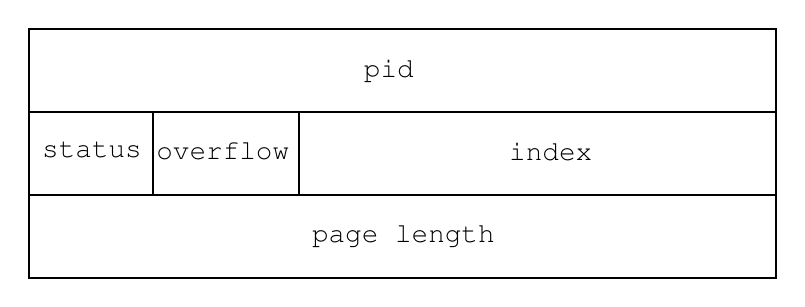
\begin{tikzpicture}[x=0.75pt,y=0.75pt,yscale=-1,xscale=1]
\draw   (190,50) -- (550,50) -- (550,90) -- (190,90) -- cycle ;
\draw   (190,90) -- (550,90) -- (550,130) -- (190,130) -- cycle ;
\draw    (250,90) -- (250,130) ;
\draw    (320,90) -- (320,130) ;
\draw   (190,130) -- (550,130) -- (550,170) -- (190,170) -- cycle ;
\draw (350,63) node [anchor=north west][inner sep=0.75pt]   [align=center] {{\fontfamily{pcr}\selectfont pid}};
\draw (195,103) node [anchor=north west][inner sep=0.75pt]   [align=left] {{\fontfamily{pcr}\selectfont status}};
\draw (250,103) node [anchor=north west][inner sep=0.75pt]   [align=left] {{\fontfamily{pcr}\selectfont overflow}};
\draw (420,103) node [anchor=north west][inner sep=0.75pt]   [align=left] {{\fontfamily{pcr}\selectfont index}};
\draw (325,143) node [anchor=north west][inner sep=0.75pt]   [align=center] {{\fontfamily{pcr}\selectfont{page length}}};
% \draw (316,63) node [anchor=north west][inner sep=0.75pt]   [align=left] {{\fontfamily{pcr}\selectfont normalized length}};
\end{tikzpicture}
\caption{Page data}
\label{fig:page_data}
\end{figure}
We discuss the mechanics of multipage segments in section 3.3.3.

\subsection{Hash Table}
Since we aren't actually given OS-level access to manipulate memory accesses, we must find another way to make it appear to the end user that all of its memory is contiguous. Unfortunately, the way we do this is by actually making memory contiguous upon access. Every time a user tries to access a new memory location, we need to check the page in that location is actually what the user expects it to be. We use a hashtable to translate apparent page numbers to where those pages are actually stored. But since our hashtable cannot interfere with our pristine block of user-level memory, we implement an open-addressed hashtable with linear probing. The hashtable is keyed by a combination of \verb|pid| and \verb|index|. This allows us to query the actual location of page \verb|index| for thread number \verb|pid|. A hashtable value is simply the actual location of this \say{virtual} page. Mechanically, a hashtable entry (see figure \ref{fig:hashtable_entry}) is 8 bytes and consists of a 32 bit process id, a 16 bit key which represents where the process thinks a page is, and a 16 bit value for where the page actually is stored in memory. The process id and 16-bit key are taken together and hashed (via linear congruential hashing) to determine the entry location in the table. Any collisions are dealt with using linear probing and tombstoning.
\begin{figure}
\centering
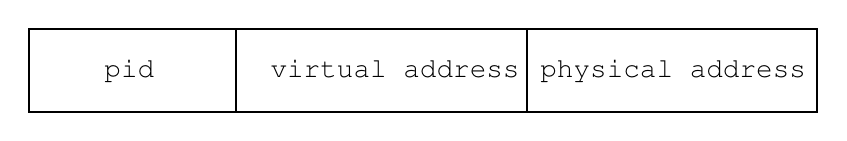
\begin{tikzpicture}[x=0.75pt,y=0.75pt,yscale=-1,xscale=1]
\draw   (190,50) -- (570,50) -- (570,90) -- (190,90) -- cycle ;
\draw    (290,50) -- (290,90) ;
\draw    (430,50) -- (430,90) ;
\draw (225,63) node [anchor=north west][inner sep=0.75pt]   [align=center] {{\fontfamily{pcr}\selectfont pid}};
\draw (305, 63) node [anchor=north west][inner sep=0.75pt]   [align=left] {{\fontfamily{pcr}\selectfont virtual address}};
\draw (435,63) node [anchor=north west][inner sep=0.75pt]   [align=left] {{\fontfamily{pcr}\selectfont physical address}};
\end{tikzpicture}
\caption{Hashtable entry}
\label{fig:hashtable_entry}
\end{figure}

\subsection{myallocate}
We continue to allocate memory using the first-fit method, but some parts of our allocation strategy needs to change to accomodate multi-page and new page allocations.

\subsubsection{New page allocations}
If a process has no pages allocated for it, we \say{virtually} allocate 8MB of free space for the process. Mechanically, we find the first free page and swap it with the first page (0), filling the page table entry for the page. Then we update page data values in two locations: First, in the page table's page data, we set the \texttt{pid} to the current process, the \texttt{status} to occupied, the \texttt{index} to the actual index of where the page is. Next, we add this actual index value and \texttt{pid}, \texttt{index} key combination to the hash table.

These steps are repeated to add new pages to a process which already has pages allocated for it. A subtle difference between this and allocating from a cold start is that the process believes it already has a full memory's worth of pages allocated that it simply needs to fill. Thus, adding new pages can be done transparently. When we allocate memory, we first check the hashtable to see if we the process has an entry for each page in the allocation range. If not, we find a free page and swap it with the allocation page, updating the pagetable and page hashtable as necessary.

We note our virtual conception of memory allows us to de-allocate pages just as easily. We discuss this further in section 3.4, but the gist is the same as for allocation.

\subsubsection{Existing page allocations}
If a process already has pages allocated for it, we traverse the process' memory space to find a free space that can service the request. If we try to access a page that has been swapped out, we simply swap it into the correct location. In this sense, our traversal is analagous to a train ride on a half-built railroad. Whenever we come across a gap in the track, we call up our friend the segfault handler to fetch a piece of track and slot it into the gap.

Unfortunately, the analogy extends further in this train ride traversal can be very slow. Since we don't maintain any free or occupied lists, we cannot know ahead of time where the free pages or free blocks are. We must go through the linkedlist from block to block, checking for free blocks of the right size. In this case, we've made a tradeoff of more compact metadata for longer execution time.

\subsubsection{Multi-page allocations}
If the allocation requires multiple pages, we do not set the normalized length within the allocation's segment metadata to match the number of segments the allocation will require. Suppose a process asks for $a = qP + r$ segments, where $P$ is the page size (in segments). We set the segment metadata for the first segment of a multi-page allocation to a non-normalized length which representing $r$, the remainder length. Then, we set the overflow flag in first page of the allocation to 1 and it's page \texttt{length} to $q$, the number of full pages taken up by the allocation. The combination of the remainder length and the page length tells us how many segments the multi-page allocation spans.

However, setting the segment metadata of a multi-page allocation to an overflow length instead of an actual segment length causes issues in accurately traversing a process' memory space. The value on its own is useless unless combined with the page data. But as it turns out, this is not an issue. The key observation is that a multi-page allocation's segment metadata will always be the last segment metadata within a page. Therefore, the segment metadata specifying overflow length (instead of actual segment length) will be the last segment metadata in a page. This is where the \verb|last| flag bit in our segment metadata comes into play. If segment is the last and the page's overflow flag is 1, then we can combine the length of the segment with the page length to accurately traverse memory. If a segment metadata is the last and page's overflow flag is 0, then the normalized length in the segment metadata is accurate and need not be combined with the page length to continue traversal.

\subsection{mydeallocate}
Again, we use our rail-road traversal of the process' memory space to find if the pointer trying to be freed was allocated. If the pointer being freed was returned upon a malloc request, it will be one byte higher than a metadata pointer. If we detect this in our traversal, we can free it very similarly to an allocation. For instance, if the allocation spanned multiple pages, we can recognize that be seeing if the pointer's respective segment metadata is the last within a page and if that page's overflow flag is set to 1.

We deallocate a page if it is entirely spanned by a free segment. That is, the segment starts before page start and ends after page start. As we noted in page allocation, this is accomplished by simply removing the page hashtable entry for it and updating the appropriate pagetable entry.

\section{Phase 3}
For this phase, we extend our memory size by 16MB with a swapfile on disk. We've set up our memory structure so that this extension is intuitive and does not require a lot of fiddling to integrate.

\subsection{Page Table and Hash Table}
%To do so, we simply create an additional page table in our disk space that has the same structure as our page table in virtual memory.  When a page is swapped out to disk, we remove its page data information from our virtual memory space and place it into our disk space. This allows us to retain the essential information that our page data structure stores even if pages have been swapped out to disk.
Because of the extra memory space that a disk provides, we are now able to allocate 4096 extra pages, as a result we need to be able to store page data and hash table information for these pages somewhere. To do so, we simply extend our page table and hash table in physical memory to index these pages as well. This represents a 3 times increase in metadata space, but this is offset by the fact that the overall ratio between metadata and virtual pages remains the same. In practice, this represents a jump from roughly 8 pages occupied for metadata (pagetable and hashtable) to 24. Recall that we have over 2000 pages in physical memory, so this monstrous blowup in metadata space corresponds to 1\% of our physical memory space.

%TODO: allocations starting at 0 now, what are the changes? 
\subsection{Swapping and Eviction}
Due to a lack of time, we chose to implement a naive eviction strategy. We treat disk as an extension of memory and we apply the same swapping strategy as in phase 2. The only difference is that we need to check if swap indices go beyond \verb|resident_pages|, the number of pages available in memory.

A discussion could be had about better eviction strategies. The LRU strategy we were originally looking at would have tied in with scheduler maintenance cycles. We would set a \say{dirty} bit upon user access, clearing the bits during a maintenance cycle. This primitive LRU scheme would allow us to be more efficient in eviction. This scheme would have fit perfectly with our pagetable metadata. Recall that a page in a 24GB memory space can be indexed in 13 bits, and our pagedata uses the top 2 bits of page \verb|index| for occupied status and overflow status. We have exactly one bit leftover for the \verb|dirty| status. Figure \ref{fig:eviction_page_data} shows this updated pagedata.

\begin{figure}
\centering
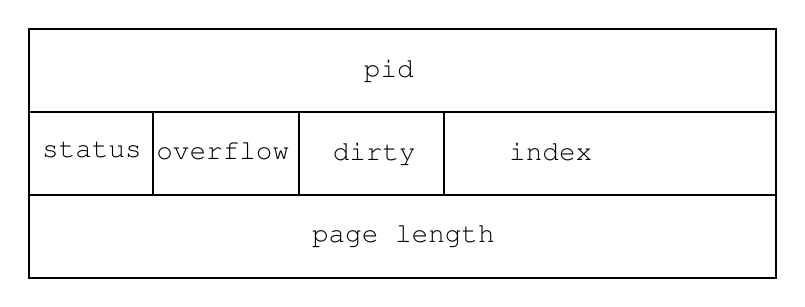
\begin{tikzpicture}[x=0.75pt,y=0.75pt,yscale=-1,xscale=1]
\draw   (190,50) -- (550,50) -- (550,90) -- (190,90) -- cycle ;
\draw   (190,90) -- (550,90) -- (550,130) -- (190,130) -- cycle ;
\draw    (250,90) -- (250,130) ;
\draw    (320,90) -- (320,130) ;
\draw    (390,90) -- (390,130) ;
\draw   (190,130) -- (550,130) -- (550,170) -- (190,170) -- cycle ;
\draw (350,63) node [anchor=north west][inner sep=0.75pt]   [align=center] {{\fontfamily{pcr}\selectfont pid}};
\draw (195,103) node [anchor=north west][inner sep=0.75pt]   [align=left] {{\fontfamily{pcr}\selectfont status}};
\draw (250,103) node [anchor=north west][inner sep=0.75pt]   [align=left] {{\fontfamily{pcr}\selectfont overflow}};
\draw (335,103) node [anchor=north west][inner sep=0.75pt]   [align=left] {{\fontfamily{pcr}\selectfont dirty}};
\draw (420,103) node [anchor=north west][inner sep=0.75pt]   [align=left] {{\fontfamily{pcr}\selectfont index}};
\draw (325,143) node [anchor=north west][inner sep=0.75pt]   [align=center] {{\fontfamily{pcr}\selectfont{page length}}};
% \draw (316,63) node [anchor=north west][inner sep=0.75pt]   [align=left] {{\fontfamily{pcr}\selectfont normalized length}};
\end{tikzpicture}
\caption{Page data}
\label{fig:eviction_page_data}
\end{figure}

\section{Engineering Challenges}
Everything we've discussed so far is how an optimal solution would be constructed. However, due to strange bugs and engineering challenges, we had to make some sacrifices after the fact. The main cause of grief is in getting swapping and memory protection to play nicely together. Namely, when we're in the scheduler we can access scheduler-specific data structures, but we need to re-protect them before handing control back to user threads. This causes two particularly nasty bugs.

\subsection{Swapping stacks while the scheduler is running}
The scheduler is meant to be called via \verb|SIGALRM|. Since it can be called at any point in time, its execution context may be plopped on top of the stack of any user thread. This is a problem. If we naively operate the scheduler on top of a user context, we cannot swap out the stack space of the old user thread with the new one, since our current execution context is running on top of the old user thread. But to swap to a new context, we must swap out all of the stack. So this requires that we run the scheduler in a separate scheduler context with a dedicated scheduler stack. We allocate this stack space as a static segment at the front of our 8BG memory block.

\subsection{The context problem}
As a rule, execution context information is not exposed to user threads, meaning if it's dynamically allocated (which it is), it must reside in scheduler memory space. However, once we execute the scheduler, we must protect scheduler space before relinquishing control to another user thread. But this means we must also protect the context we wish to run, so \verb|swapcontext| will segfault. Even worse, we won't be able to catch the signal and handle it gracefully, so any call to \verb|swapcontext| will crash the whole program. This is a particularly nasty problem to which we found no good solution. Either we employ a two-sided heap system for normal vs scheduler memory (to ensure we never need to protect scheduler memory) or we declare thread contexts outside of the memory protection scope. In the interest of time, we chose the latter. We pre-allocate a portion of our memory space for a static array of \verb|ucontext_t| structs. In our final implementation, we give 200 pages, the equivalent of roughly 800 total threads. This is the hard limit on concurrent threads created, since we can delare context information in neither user nor scheduler memory space and instead must declare it in the static array.

One may argue that this a reasonable thread limit, and we would be inclined to agree with that argument. However, the main drawback is that these 200 pages must remain in \say{global} memory, reducing the number of physical pages avaiable for allocation by 200. This is a substantial loss of available physical memory, representing almost 10\% of the 8GB memory allocation.

\section{Further Work}
Due to the time crunch, we were unable to implement a non-naive eviction and swapping system. Any of the LRU methods discussed in class (second-chance, timestamp, etc.) would be more efficient. In addition, our allocation is inefficient. Since we don't keep a free list, we need to traverse potentially all of memory to find a free block or say we are out of memory. In a purely memory-based system, this might be passable. But a traversal in phase C can require arbitrarily many IOs to swap pages from disk. This is an inherent limitation of not having free lists or more metadata. With more time, we may be able to redesign our memory structure to reduce this traversal IO cost.

\end{document}

% List of tex snippets:
%   - tex-header (this)
%   - R      --> \mathbb{R}
%   - Z      --> \mathbb{Z}
%   - B      --> \mathcal{B}
%   - E      --> \mathcal{E}
%   - M      --> \mathcal{M}
%   - m      --> \mathfrak{m}({#1})
%   - normlp --> \norm{{#1}}_{L^{{#2}}}